\chapterauthor{Author Name1}{Affiliation text1}
\chapterauthor{Author Name2}{Affiliation text2}
\chapterauthor{Author Name3}{Affiliation text3}
\chapterauthor{Author Name4}{Affiliation text4}

\chapter{Multi objective evolutionary algorithms applied to Protein Structure Prediction Problem}

\section{Introduction} \label{sec:intro}

%Objetivos

%Contribuições

\section{Protein Structure Prediction} \label{sec:proteinfolding}


Proteins are macromolecules made out of  twenty different amino acids, also referred to as residues. An amino acid has a peptide backbone and a distinctive side chain group. The peptide bond is defined by an amino group and a carboxyl group connected to an alpha carbon to which  a hydrogen and side chain group are attached.

Amino acids are combined to form sequences which are considered the primary structure of the peptides or proteins. The secondary structure is the locally ordered structure brought about via hydrogen bounding mainly within the peptide backbone. The most common secondary structure elements in proteins are the alpha helix and the beta sheet. The tertiary structure is the global folding of a single polypeptide chain.

Under specific conditions, the protein sequence folds into a unique native 3-d structure. Each possible protein fold has associated energy. The \emph{thermodynamic hypothesis} states that the native structure of a protein is the one for which the free energy achieves the global minimum. Based on this hypothesis, many methods that search for the protein native structure define an approximation of the protein energy and use optimization algorithms that look for the protein fold that minimizes this energy. These approaches mainly differ in the type of energy approximation employed and in the characteristics of the protein modeling.


\subsection{The HP Model}


The HP model considers two types of residues:  hydrophobic (H) residues  and hydrophilic or polar (P) residues. A protein is considered a sequence of these two types of residues, which are located in regular lattice models forming self-avoided paths. Given a pair of residues, they are considered neighbors if they are adjacent  either in the chain (connected neighbors) or  in the lattice but not connected in the chain (topological neighbors).


\begin{figure}[htb] \label{fig:PROTEXAM}
	\centering
	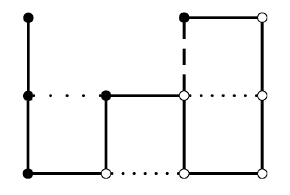
\includegraphics[scale=0.7]{figures/protein_example.png}
	\caption{One possible configuration of  sequence $HHHPHPPPPPH$ in the HP model. There is one $HH$ (represented by a dotted line with wide spaces), one $HP$ (represented by a dashed line) and  two $PP$  (represented by dotted lines) contacts.}
\end{figure}


The total number of topological neighboring positions in the lattice ($z$) is called the lattice coordination number.


For the HP model, an energy function that  measures the interaction between topological  neighbor residues is defined  as  $\epsilon_{HH}=-1$ and $\epsilon_{HP}=\epsilon_{PP}=0$. The HP problem consists of finding the solution that minimizes the total energy. In the linear representation of the sequence, hydrophobic residues are represented with the letter H and polar ones, with P. In the graphical representation, hydrophobic proteins are represented  by black beads and polar proteins, by white beads. Figure~\ref{fig:PROTEXAM} shows the graphical representation of a possible configuration for  sequence  $HHHPHPPPPPH$. The energy that the HP model associates with this configuration is $-1$ because there is only one $HH$ contact, arisen between the second and fifth residues.


Different heuristic approaches have been developed to decrease the computational complexity related to the protein structure determination process. Between this approaches, there are studies that explore the protein structure prediction combined with evolutionary algorithms like for example, the author of \cite{li2012genetic} proposed an mono objective EA (Evolutionary Algorithm) working with a local search strategy for the PSP Problem using the simplified model Hydrophobic-Polar 2D (2D-HP).


The authors of \cite{lin2011protein} applied a hybrid genetic-based PSO algorithm to 3D HP model with relative representation, optimizing the crossover and mutation operators to improve results in the Protein Folding process.


In \cite{custodio2014multiple} is proposed a Multiple minima genetic algorithm for PSP. The algorithm includes a phenotype based crowding mechanism fo the maintenance of useful diversity which increase the population's performance and granted the algorithm multiple solutions capabilities.


Then \cite{soares2011investigating} proposed an multi objective algorithm in tables and compares its performance with the NSGAII \cite{deb2002fast}, optimizing two energy functions, both very important for the the folding process: the van der Walls and Electrostatic functions.


The author of \cite{gabriel2012algoritmos} also proposes the using of a multi objective algorithm in tables, similar to the proposed method by \cite{soares2011investigating}, however, using the HP model for the representation and solution evaluation.


\section{Multi-objective Optimization} \label{sec:optimization}


Evolutionary Algorithm (EA) is a optimization and search technique, highly parallel, inspired by the Darwinian principle of natural selection and genetic reproduction. The nature principles that inspire the EAs are simple. According to the theory of C, Darwin, the principle of natural selection favors individuals with high fitness, therefore, with high probability of reproduction. Individuals with more descendants have more chance to perpetuate their genetic code in future generations. The genetic codes is what gives the identity of each individual and are represented in the chromosomes. These principles are used in the construction of computational algorithms, that searches for better solutions given a specific problem by the evolution of a population of solutions coded in artificial chromosomes -- data structures used to represent a feasible solution for a given problem in the algorithm execution \cite{pacheco1999algoritmos}.


Real world problems commonly have multiple objectives to minimized/maximized and are present in most knowledge areas. To optimize multi objective problems, are considered two or more objectives witch usually are conflicting. To these problems is impossible to find one unique solution. A set of solutions is reached evaluating the Pareto dominance relation \cite{pareto} between the solutions. The main objective is to find the solutions that are non-dominated by any other. A solution dominates other, if and only if, it was better in at least one of the objectives, without being worst in any of the objectives. The set of non-dominated solutions constitutes the Pareto Front. Finding the the real Pareto Front is a NP-hard problem \cite{fonseca2005tutorial}, this way, the objective is to find a good approximation of this front.


Multi-Objective Evolutionary Algorithms (MOEAS) are extensions of EAs to multi objective problems that applies the concepts of Pareto dominance to create different strategies to evolve and diversify the solutions. In this work were used two MOEAs: NSGAII \cite{deb2002fast} and IBEA \cite{zitzler2004indicator}.


\subsection{Non-dominated sorting Genetic Algorithm II}


The main characteristic of this algorithm is a strong elitism mechanism, classifying at each generation every solution in different fronts according with the non-dominance relation (line 15 of Algorithm \ref{alg:nsgaII}). After the classification, solutions from the first front, are non-dominated by any other solution. Solutions from the second front are dominated only by the solutions of the first front, and so on. For solutions of the same front, the algorithm uses a Crowding Distance operator to calculate how distant are the neighbors of a given solution (line 19 of Algorithm \ref{alg:nsgaII}). Solutions with high values of Crowding Distance have priority, because they will contribute more to the population's diversity. The binary tournament selects solutions from the small front with the higher values of Crowding Distance. A new population is generated using the crossover and mutation operators (line 25 of Algorithm \ref{alg:nsgaII}).


\begin{algorithm}[htb]
	\begin{algorithmic}[1]
		\State{$N \gets$ Population Size}
		\State{$T \gets$ Max evaluations}
		\State{$P_0 \gets CreatePopulation(N);$}
		\State{$CalculateFitness(P_0);$}
		\State{$FastNonDominatedSort(P_0);$}
		\State{$Q_0 \gets 0$}
		\While{$Q_0 < N$}
			\State{$Parents \gets BinaryTournament(P_0);$}
			\State{$Children \gets CrossoverMutation(Parents);$}
			\State{$Q_0 \gets Children$}
		\EndWhile
		\State{$CalculateFitness(Q_0);$}
		\State{$t \gets 0$}
		\While{$t < T$}
			\State{$R_t \gets P_t \cup Q_t;$}
			\State{$Fronts \gets FastNonDominatedSort(R_t);$}
			\State{$P_{t+1} \gets 0$}
			\State{$i \gets 0$}
			\While{$P_{t+1} + Front_i  < N$}
				\State{$CrowdingDistanceAssignment(Front_i);$}
				\State{$P_{t+1} \gets P_{t+1} \cup Front_i$}
				\State{$i \gets i + 1$}
			\EndWhile
			\State{$CrowdingDistanceSort(Front_i);$}
			\State{$P_{t+1} \gets P_{t+1} \cup Front_i[1:(N -P_{t+1})]$}
			
			\State{$Parents \gets BinaryTournament(P_{t+1});$}
			\State{$Q_{t+1} \gets CrossoverMutation(Parents);$}
			\State{$t \gets t +1$}
		\EndWhile
		\State{\Return{$P \gets$ Set of non-dominated solutions.}}
	\end{algorithmic}
	\caption{NSGAII}
	\label{alg:nsgaII}
\end{algorithm}


\subsection{IBEA (Indicator-Based Evolutionary Algorithm)}


In the multi-objective optimization context, optimizing consists in find a front with a good approximation to the true Pareto front. However, there is no general definition about what is the true Pareto front. This way, indicators have been used to evaluate the quality of a approximation front. The \textit{hypervolume} is a example of indicator to the evaluation and comparison of fronts.


The IBEA is an algorithm that considers the optimization by the use of quality indicators. The indicator is the way used to evaluate the non-dominated set of solutions \cite{figueiredo2013algoritmo}. To use the IBEA it is necessary define which indicator will be used to associate each ordered pair of solutions to a scalar value. One of the most used indicators is the \textit{hypervolume} due to its capacity of evaluate the convergence and diversity at the same time of the search process \cite{ishibuchi2008evolutionary}.


\begin{equation} \label{eq:ibea_fitness}
F(x_i) = \sum_{x_j \in (P-x_i)} {-e^\frac{-I_{Hy}(x_j,x_i)}{k}}
\end{equation}


For the IBEA fitness calculation (Equation \ref{eq:ibea_fitness}), $k$ is a parameter commonly used with a value of 0.05. The value for $F(x_i)$ corresponds to a quality loss measure of the approximation to the Pareto front if the solution $x_i$ was removed of the population \cite{figueiredo2013algoritmo}, based on the value of the quality indicator $I_{Hy}$, in this case, the \textit{hypervolume}. Based on the fitness calculation described above, the basic IBEA algorithm consists in iteratively do the selection (line 10 of Algorithm \ref{alg:ibea}), crossover, mutation (line 11 of Algorithm \ref{alg:ibea}) and environment selection, removing the worst individual from the population and updating the values of fitness of the remaining individuals (lines 4 to 8 of Algorithm \ref{alg:ibea}).


\begin{algorithm}[htb]
	\begin{algorithmic}[1]
	\State{$N \gets$ Population Size}
	\State{$T \gets$ Max Evaluations}
	\State{$k \gets$ Scale factor of Fitness}
	
	\State{$P \gets$ CreatePopulation($N$);}
	\State{$m \gets 0$}
	\State{CalculateFitness($P$);}
	
	\While{$m \ge T$ or other stop criterion is reached}
		
		\State{$\overline P \gets$ BinaryTournament($P$);}
		\State{$P \gets$ CrossoverMutation($\overline P$);}
		\State{$m \gets m+1$}
		
		\While{Size($P$) $> N$}
			\State{$x^* \gets$ WorstIndividualByFitness();}
			\State{RemoveFromPopulation($x^*$, $P$);}
			\State{CalculateFitness($P$);}
		\EndWhile
	
	\EndWhile
		\State{\Return{$P \gets$ Set of non-dominated solutions}}
	
	\end{algorithmic}
	\caption{IBEA}
	\label{alg:ibea}
\end{algorithm}


\footnotetext[1]{\textit{Hypervolume}: Proposed quality indicators used in the study of \cite{zitzler1998multiobjective}, denoted as the "size of the covered search space". This indicator has two important advantages in relation to others \cite{zitzler2007hypervolume}: 1 - Sensitive to any kind of improvement in the approximation set in relation to other set. 2 - As result of 1, the indicator guarantee that for any approximation set $A$ that has high values of hypervolume, also has all the solutions of the true Pareto front.}


\section{Proposed method}


The proposed method consists in the application of the algorithms NSGAII and IBEA to the PSP problem using the relative representation applied to the HP model. The multi-objective optimization framework jMetal \cite{jMetal} was used, it presents implementation of the used MOEAs and a easy way to personalize them. To evaluate the generated solutions, a evaluation mechanism was implemented considering two objectives:


\begin{enumerate}
	\item Maximize the number of topological neighbors HH (main objective);
	\item Minimize the maximum euclidean distance between residues (secondary objective).
\end{enumerate}


The first objective guide the search aiming find a solution that generates a structure where the energy value is minimum (maximizing the number of topological neighbors HH), this way, obtaining a structure closer of the native conformation of the protein. The second objective allows to differ solutions with the same value of energy but with different compression degrees. The more compact was the max value of euclidean distance, more compact will be the generated conformation.


The chromosomes are represented by integer vectors where the genes specify which direction, related to the previous residue, the next one should be placed. The genes can assume one of three values 0, 1 and 2, where 0 means the next residue should be placed at right of the previous one, 1 means the next residue should be placed in front of the previous and 2 means the next residue should be placed at left of the previous one. The Figure \ref{fig_sim} demonstrate a example of a possible chromosome to a chain of 10 residues and its generated conformation.


\begin{figure}[ht]
	\centering
	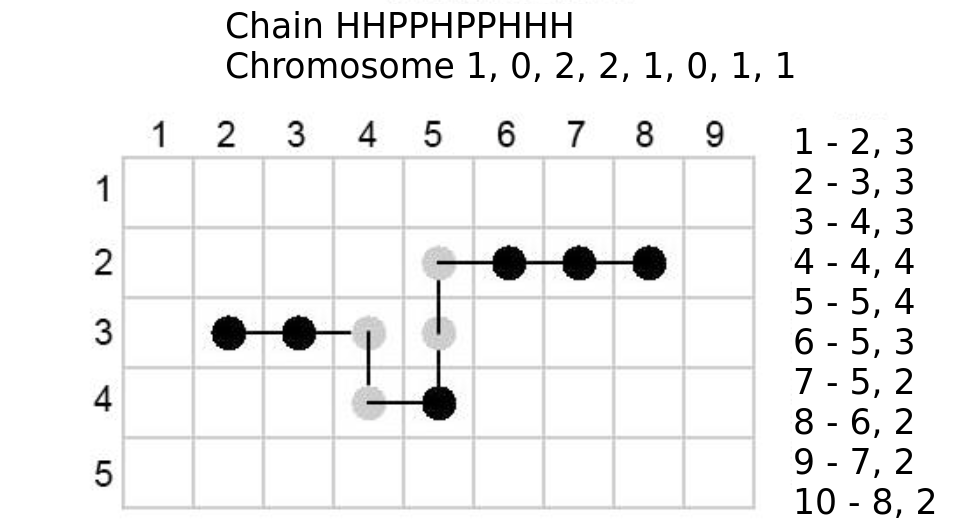
\includegraphics[width=2.5in]{figures/figure3.png}
	\caption{Example of a conformation generated by a chromosome with relative representation.}
	\label{fig_sim}
\end{figure}


The relative representation it is subject to the generation of infeasible solutions using the HP model. A solution is considered infeasible when a residue 'collides' with another already placed on the lattice. A simple mechanism for repairing these situations was developed, the code can be seen in the Algorithm \ref{algo:reparacao}.


\begin{algorithm}[h]
	Obtains the direction the next residue should be placed.\\
	Verifies if this direction will cause collision.\\
	If the a collision is identified, a new direction is used.\\
	Repeat the step 2 and 3, until be possible to place the next residue, or if all directions were tested and cause collisions.\\
	If was possible to place the next residue, the mechanism reached success, if not, the solution is considered infeasible and it will be penalized in the evaluation process.
	\caption{Mechanism to repair infeasible solutions}
	\label{algo:reparacao}
\end{algorithm}


This mechanism was implemented because in early experiments was observed that the number of infeasible solutions was too big. It is necessary mention that the even with the mechanism to repair solutions, there are still infeasible solutions because the mechanism can't always repair. Yet, infeasible solutions are penalized by subtracting the number of collisions to the quantity of topological neighbors.


To evaluate and compare the performance of the multi-objective algorithms, quality indicators are commonly used. In this study was used the hypervolume indicator, which considers the volume of the search space dominated by the true front \cite{zitzler2003performance}. The high the hypervolume is, better the quality of the front found by one of the algorithms.


%Proposta antiga vs proposta nova

\section{Experiments}

\section{Conclusion}